\section{Results}\label{sec:results}

\subsection{The Run}\label{sec:run}

The main grid measured \RunProcesses{} processes of \RunArms{} arms. Of these, \RunOk{} ended with
every answer right, \RunRefused{} were refusals of a table, and \RunDeclared{} differed from the
expected answers as their arm's declaration allows. No cell failed and no process exceeded its
budget. The agreement pass stopped \VerifyCut{} processes at its budget, \VerifyCutActix{} of them
actix-router at $m=\SizeHundredThousand$. The repeated check of Section~\ref{sec:deviation} found all
\VerifyRepeatAgreed{} right on every query.

A competitor was absent from a cell only by refusal or by declaration. On \shape{wild}, uWebSockets is
incomparable and Pistache refuses the tables, because its splat matches one segment only. So
\HOneCompetitorsWildTen{} competitors take part. On \shape{mixed-overlap}, Boost.URL, gin and r3 are
incomparable and httprouter refuses the tables, so \HOneCompetitorsMixedOverlapTen{} take part.
Elsewhere all sixteen do. In no cell of H1 did v2 or the fastest competitor run on a prefix of the
ring.

\subsection{H1: Lookup Time}\label{sec:hone}

H1 \HOneVerdict. Of the \HOneCells{} cells, \HOnePassed{} pass under both computations, where
\HOneNeed{} were needed, and no tested cell's upper bound exceeds \HOneCapTwo. The largest is
\HOneMaxHigh. The two computations agree in every cell. Of the cells that pass, \HOneSuperior{} also
pass the superiority test. In those cells, and in the setting of Section~\ref{sec:host}, v2 is faster than the
fastest competitor. There it took \HOneSupRatioMin{} to \HOneSupRatioMax{} of that competitor's time.
Figure~\ref{fig:hone} shows every cell, and Table~\ref{tab:hone} gives the numbers.

\begin{figure}[htbp]
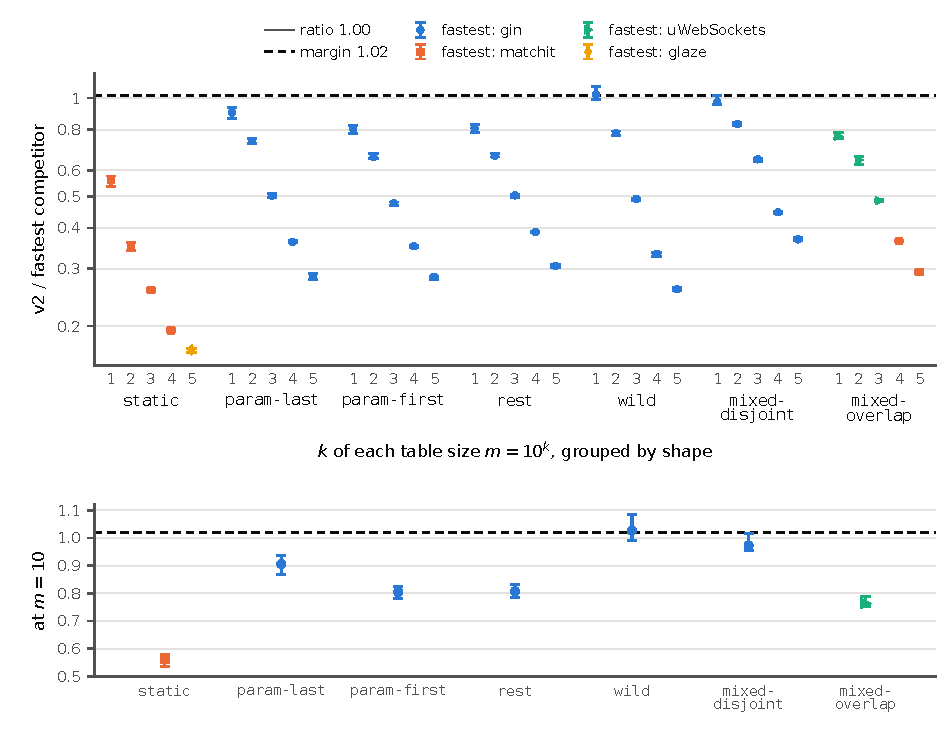
\includegraphics[width=\linewidth]{fig/fig_h1.pdf}
\caption{H1 per cell: v2's time over the fastest competitor's, as the median over the
\RoundTwoReps{} pairs of the per-pair ratio, with its \Level\% BCa interval. Colour and marker name
the fastest competitor. The dashed line is the margin \Margin, and the solid line the ratio
\SupMargin. The upper panel shows every cell on a logarithmic axis. The lower panel shows the cells at
$m=\SizeTen$ on a linear axis, where the two lines are told apart.\label{fig:hone}}
\end{figure}

\begin{table}[htbp]
\caption{H1 per cell. $n$ is the number of competitors in the cell. v2 and F are the medians over
processes of v2's and the fastest competitor's time per lookup. ``Ratio'' is the median of the per-pair
ratios, with its \Level\% BCa interval. $X$ counts the pairs below \Margin. $p_{\mathrm{NI}}$ and
$p_{\mathrm{S}}$ are the larger of the two Holm-adjusted p of non-inferiority and of superiority. NI
and S say whether the cell passes each.\label{tab:hone}}
\begin{adjustwidth}{-\extralength}{0cm}
\centering\footnotesize\setlength{\tabcolsep}{3pt}
\begin{tabular}{@{}llllrrrlrrlrl@{}}
\toprule
\textbf{Shape} & $m$ & \textbf{Fastest} & $n$ & \textbf{v2 (ns)} & \textbf{F (ns)} & \textbf{Ratio} &
\textbf{\Level\% BCa} & $X$ & $p_{\mathrm{NI}}$ & \textbf{NI} & $p_{\mathrm{S}}$ & \textbf{S} \\
\midrule
\HOneRowStaticTen \\ \HOneRowStaticHundred \\ \HOneRowStaticThousand \\ \HOneRowStaticTenThousand \\
\HOneRowStaticHundredThousand \\ \addlinespace
\HOneRowParamLastTen \\ \HOneRowParamLastHundred \\ \HOneRowParamLastThousand \\
\HOneRowParamLastTenThousand \\ \HOneRowParamLastHundredThousand \\ \addlinespace
\HOneRowParamFirstTen \\ \HOneRowParamFirstHundred \\ \HOneRowParamFirstThousand \\
\HOneRowParamFirstTenThousand \\ \HOneRowParamFirstHundredThousand \\ \addlinespace
\HOneRowRestTen \\ \HOneRowRestHundred \\ \HOneRowRestThousand \\ \HOneRowRestTenThousand \\
\HOneRowRestHundredThousand \\ \addlinespace
\HOneRowWildTen \\ \HOneRowWildHundred \\ \HOneRowWildThousand \\ \HOneRowWildTenThousand \\
\HOneRowWildHundredThousand \\ \addlinespace
\HOneRowMixedDisjointTen \\ \HOneRowMixedDisjointHundred \\ \HOneRowMixedDisjointThousand \\
\HOneRowMixedDisjointTenThousand \\ \HOneRowMixedDisjointHundredThousand \\ \addlinespace
\HOneRowMixedOverlapTen \\ \HOneRowMixedOverlapHundred \\ \HOneRowMixedOverlapThousand \\
\HOneRowMixedOverlapTenThousand \\ \HOneRowMixedOverlapHundredThousand \\
\bottomrule
\end{tabular}
\end{adjustwidth}
\end{table}

gin was the fastest competitor in \HOneFastestGinCells{} cells, matchit in
\HOneFastestMatchitCells, uWebSockets in \HOneFastestUWebSocketsCells{} and glaze in
\HOneFastestGlazeCells. The gap grows with the table. On \shape{static}, v2's time rose from
\HOneVtwoNsStaticTen~ns at $m=\SizeTen$ to \HOneVtwoNsStaticHundredThousand~ns at
$m=\SizeHundredThousand$. Over the same sizes, the fastest competitor's rose from
\HOneFastestNsStaticTen~ns to \HOneFastestNsStaticHundredThousand~ns.

\runin{\shape{wild} at $m=\SizeTen$.} This is the one cell that does not pass. Its ratio against
gin is \HOneRatioWildTen, with the interval [\HOneLowWildTen, \HOneHighWildTen]. Only
\HOneSignXWildTen{} of \RoundTwoReps{} pairs are below \Margin, and the Holm-adjusted p is
$\HOnePHolmWildTen$. So the paper claims neither ``not slower'' nor ``faster'' in this cell. The loss is
in a single cell, so the claim narrows at that cell only, as the pre-specification requires.
\shape{wild} passes both tests at every other size. Section~\ref{sec:gin} discusses this cell.

\runin{\shape{mixed-disjoint} at $m=\SizeTen$.} This cell passes non-inferiority and not
superiority. Its ratio against gin is \HOneRatioMixedDisjointTen, with the interval
[\HOneLowMixedDisjointTen, \HOneHighMixedDisjointTen]. Of the sixteen pairs,
\HOneSignXMixedDisjointTen{} are below \Margin, but only \HOneSignXSupMixedDisjointTen{} below
\SupMargin. So v2 is not slower than gin here,
and the paper does not call it faster.

Whether this cell passes depends on the family that Holm's procedure adjusts it in. Before the
repeated check, \HOneAsIsUntested{} cells at $m=\SizeHundredThousand$ could not be tested, because
processes of actix-router were not verified on every query. Each entered Holm with a p of one, and
\HOneAsIsPassed{} of the \HOneAsIsTested{} tested cells passed. This cell's raw sign-test p is
$\HOnePSignRawMixedDisjointTen$ in both analyses. With the untested cells at the bottom of the order,
its Holm multiplier was \HOneHolmMultiplierBeforeMixedDisjointTen, so its adjusted p was
\HOnePSignHolmBeforeMixedDisjointTen, above \Alpha. Once those cells were tested, their p were small. The
cell's multiplier fell to \HOneHolmMultiplierAfterMixedDisjointTen, and its adjusted p to
$\HOnePSignHolmMixedDisjointTen$. Its bootstrap p moved as well, from
\HOnePBootRawBeforeMixedDisjointTen{} to $\HOnePBootRawMixedDisjointTen$ before adjustment, and from
\HOnePBootHolmBeforeMixedDisjointTen{} to $\HOnePBootHolmMixedDisjointTen$ after it. One generator serves the tested cells in the
family's order, so more tested cells change the draws of every later cell. The cell's ratio and
interval do not depend on the family.

\subsection{H2: Work per Lookup}\label{sec:htwo}

H2 \HTwoVerdict. It holds in \HTwoHeld{} of \HTwoJudged{} cells (Table~\ref{tab:htwo}). v2 took fewer
branch misses than the median competitor in every cell, with or without the cut competitors,
\HTwoCutArms. The \HTwoLost{} losses are net instructions against gin, at \HTwoLostCells. At
\shape{param-last}, v2 ran \HTwoVtwoNetParamLastTen{} net instructions per lookup against gin's
\HTwoFastestNetParamLastTen. At \shape{mixed-disjoint}, it ran \HTwoVtwoNetMixedDisjointTen{} against
\HTwoFastestNetMixedDisjointTen. The pre-specification predicted the second loss and not the first.

The memory-side counters per lookup of the losing cells are small for both arms. At
\shape{param-last}, v2 took \HTwoVtwoLOneDParamLastTen{} L1d misses, \HTwoVtwoLTwoParamLastTen{} L2
misses and \HTwoVtwoDtlbParamLastTen{} DTLB misses. gin took \HTwoFastestLOneDParamLastTen,
\HTwoFastestLTwoParamLastTen{} and \HTwoFastestDtlbParamLastTen. At \shape{mixed-disjoint}, v2 took
\HTwoVtwoLOneDMixedDisjointTen, \HTwoVtwoLTwoMixedDisjointTen{} and \HTwoVtwoDtlbMixedDisjointTen,
and gin \HTwoFastestLOneDMixedDisjointTen, \HTwoFastestLTwoMixedDisjointTen{} and
\HTwoFastestDtlbMixedDisjointTen. In both cells v2 still took fewer branch misses than the median
competitor, and by H1 it was not slower than gin.

\begin{table}[htbp]
\caption{H2 per cell: instructions per lookup, net of the null of each arm's own loop and raw, and
branch misses per lookup. ``Median'' is the median competitor's branch misses. The next column leaves
out the competitors whose passes were cut, where any were.\label{tab:htwo}}
\begin{adjustwidth}{-\extralength}{0cm}
\centering\footnotesize\setlength{\tabcolsep}{3.5pt}
\begin{tabular}{@{}lllrrrrrrrl@{}}
\toprule
& & & \multicolumn{2}{c}{\textbf{Net instructions}} & \multicolumn{2}{c}{\textbf{Raw instructions}} &
\multicolumn{3}{c}{\textbf{Branch misses}} & \\
\cmidrule(lr){4-5}\cmidrule(lr){6-7}\cmidrule(lr){8-10}
\textbf{Shape} & $m$ & \textbf{Fastest} & \textbf{v2} & \textbf{Fastest} & \textbf{v2} &
\textbf{Fastest} & \textbf{v2} & \textbf{Median} & \textbf{Uncut} & \textbf{Holds} \\
\midrule
\HTwoRowStaticTen \\ \HTwoRowStaticHundred \\ \HTwoRowStaticThousand \\ \HTwoRowStaticTenThousand \\
\HTwoRowStaticHundredThousand \\ \addlinespace
\HTwoRowParamLastTen \\ \HTwoRowParamLastHundred \\ \HTwoRowParamLastThousand \\
\HTwoRowParamLastTenThousand \\ \HTwoRowParamLastHundredThousand \\ \addlinespace
\HTwoRowParamFirstTen \\ \HTwoRowParamFirstHundred \\ \HTwoRowParamFirstThousand \\
\HTwoRowParamFirstTenThousand \\ \HTwoRowParamFirstHundredThousand \\ \addlinespace
\HTwoRowRestTen \\ \HTwoRowRestHundred \\ \HTwoRowRestThousand \\ \HTwoRowRestTenThousand \\
\HTwoRowRestHundredThousand \\ \addlinespace
\HTwoRowWildTen \\ \HTwoRowWildHundred \\ \HTwoRowWildThousand \\ \HTwoRowWildTenThousand \\
\HTwoRowWildHundredThousand \\ \addlinespace
\HTwoRowMixedDisjointTen \\ \HTwoRowMixedDisjointHundred \\ \HTwoRowMixedDisjointThousand \\
\HTwoRowMixedDisjointTenThousand \\ \HTwoRowMixedDisjointHundredThousand \\ \addlinespace
\HTwoRowMixedOverlapTen \\ \HTwoRowMixedOverlapHundred \\ \HTwoRowMixedOverlapThousand \\
\HTwoRowMixedOverlapTenThousand \\ \HTwoRowMixedOverlapHundredThousand \\
\bottomrule
\end{tabular}
\end{adjustwidth}
\end{table}

\subsection{H3: No Allocation}\label{sec:hthree}

H3 \HThreeVerdict. In all \HThreeProcesses{} processes of v2 over the \HOneCells{} cells, a lookup made
no heap allocation. The compile-time arm, in its \HThreeCtProcesses{} processes, and the ablation arm,
in its \HThreeAblationProcesses, made none either.

\subsection{H4: Build Time and Memory}\label{sec:hfour}

H4 \HFourVerdict. It fails in \HFourLost{} cells, all on build time: \shape{static} and
\shape{param-first} at $m=\SizeTenThousand$ and \SizeHundredThousand. There v2's build took
\HFourLostRatioMin{} to \HFourLostRatioMax{} times the median competitor's (Table~\ref{tab:hfour}).
The other two bounds hold in every cell. v2's slowest build at $m=\SizeHundredThousand$ took
\HFourBuildMaxMs~ms, below \BuildLimitSeconds~s. Its table held \HFourHeapRatioMin{} to
\HFourHeapRatioMax{} times the heap bytes of the smallest competitor, within the factor
\HeapFactor. As pre-specified, H4's claim is not made.

\begin{table}[htbp]
\caption{H4 per cell. Build times are medians over processes of each process's median build, in
microseconds. ``Median'' is the median competitor's build time. Heap bytes are those the built table
holds. ``Smallest'' is the competitor with the fewest.\label{tab:hfour}}
\begin{adjustwidth}{-\extralength}{0cm}
\centering\footnotesize\setlength{\tabcolsep}{4pt}
\begin{tabular}{@{}llrrrrllll@{}}
\toprule
& & \multicolumn{2}{c}{\textbf{Build ($\mu$s)}} & \multicolumn{3}{c}{\textbf{Heap bytes}} &
\multicolumn{3}{c}{\textbf{Holds}} \\
\cmidrule(lr){3-4}\cmidrule(lr){5-7}\cmidrule(lr){8-10}
\textbf{Shape} & $m$ & \textbf{v2} & \textbf{Median} & \textbf{v2} & \textbf{Smallest} & & \textbf{Build} &
\textbf{Heap} & \textbf{Cell} \\
\midrule
\HFourRowStaticTen \\ \HFourRowStaticHundred \\ \HFourRowStaticThousand \\ \HFourRowStaticTenThousand \\
\HFourRowStaticHundredThousand \\ \addlinespace
\HFourRowParamLastTen \\ \HFourRowParamLastHundred \\ \HFourRowParamLastThousand \\
\HFourRowParamLastTenThousand \\ \HFourRowParamLastHundredThousand \\ \addlinespace
\HFourRowParamFirstTen \\ \HFourRowParamFirstHundred \\ \HFourRowParamFirstThousand \\
\HFourRowParamFirstTenThousand \\ \HFourRowParamFirstHundredThousand \\ \addlinespace
\HFourRowRestTen \\ \HFourRowRestHundred \\ \HFourRowRestThousand \\ \HFourRowRestTenThousand \\
\HFourRowRestHundredThousand \\ \addlinespace
\HFourRowWildTen \\ \HFourRowWildHundred \\ \HFourRowWildThousand \\ \HFourRowWildTenThousand \\
\HFourRowWildHundredThousand \\ \addlinespace
\HFourRowMixedDisjointTen \\ \HFourRowMixedDisjointHundred \\ \HFourRowMixedDisjointThousand \\
\HFourRowMixedDisjointTenThousand \\ \HFourRowMixedDisjointHundredThousand \\ \addlinespace
\HFourRowMixedOverlapTen \\ \HFourRowMixedOverlapHundred \\ \HFourRowMixedOverlapThousand \\
\HFourRowMixedOverlapTenThousand \\ \HFourRowMixedOverlapHundredThousand \\
\bottomrule
\end{tabular}
\end{adjustwidth}
\end{table}

\subsection{H5: Checked When Compiled, Correct When Run}\label{sec:hfive}

H5 holds in all three parts. (a) RegexMatcher's suite at the measured commit holds the \NegCases{}
negative-compilation cases, one test each. Each expects the compilation to fail and checks that the
diagnostic names the reason. Under each of the three sanitizers on L, all \HFiveATests{} tests of the
suite passed. (b) v2 answered all \HFiveBLookups{} lookups of the probes as the rules require.
Table~\ref{tab:probes} shows every arm. v1 behind its wrapper fails two probes; this decides
nothing. Of the competitors, only matchit and path-tree pass every probe,
as v2 does. (c) The minimal server's suite checks that the GET route serves HEAD on a path that only
GET routes match, without content. It also checks that a HEAD route wins over that fallback, and that
Allow lists HEAD whenever it lists GET. The suite passed under each of the three sanitizers on L.

\begin{table}[htbp]
\caption{The probes of the path rules on every arm. S$\to$P and P$\to$S register a literal route
before a parameter route and after it. ``pchar'' sends every pchar in a parameter, ``raw'' a path
that differs only in the case of a percent escape. ``catch-all'' and ``empty'' test the rules on
remainders and empty segments, ``slash'' a trailing slash, and 405 a path of another method.
$\checkmark$: every lookup right; $\times$: at least one wrong; $\circ$: the arm refused the probe's
routes.\label{tab:probes}}
\centering\footnotesize\setlength{\tabcolsep}{4pt}
\begin{tabular}{@{}lcccccccc@{}}
\toprule
\textbf{Arm} & S$\to$P & P$\to$S & pchar & raw & catch-all & empty & slash & 405 \\
\midrule
\ProbeArms
\bottomrule
\end{tabular}
\end{table}

\subsection{H6: The Client Sees the Difference}\label{sec:hsix}

H6 holds. Part (a) \HSixAVerdict{} in \HSixAHeld{} of \HSixCells{} cells, and part (b) \HSixBVerdict{}
in \HSixBHeld{} of \HSixCells{} (Table~\ref{tab:hsix}). Every cell stopped at \HSixMinPairs{} valid
pairs, and none of the \HSixWindows{} windows was invalid. With v2 the server answered
\HSixVtwoRpsMin{} to \HSixVtwoRpsMax{} requests per second in every cell. At $m=\SizeTen$ the lower
bounds of the ratio over v1 ranged from \HSixLowMinTen{} to \HSixLowMaxTen. At \shape{rest} with
$m=\SizeTenThousand$, v1's lookup dominated its server's time, and the ratio was
\HSixRatioRestTenThousand. There v1's lookup time in the main grid rests on a prefix of
\HSixVOnePrefixRestTenThousand{} of the \RingSize{} queries, as the pre-specification allows.

The lower bounds of the carry-over ranged from \HSixCarryLowMin{} to \HSixCarryLowMax, all above
\CarryBound. The null arm took \HSixNullUsMin{} to \HSixNullUsMax~$\mu$s per request. The measured
ratio was \HSixPredMin{} to \HSixPredMax{} times the ratio that the lookup times predict. In every
cell every pair favoured v2 and carried at least \CarryBound, so each sign test gives \HSixSignMinP.
H6 compares v2 with v1 in the paper's own server. It says nothing about the competitors, nor about a
full framework.

\begin{table}[htbp]
\caption{H6 per cell, over loopback with the minimal server. Rates are the medians over pairs, in
requests per second. ``Low'' is the lower bound of the \Level\% BCa interval. $D_{T0}$ and
$D_{\mathrm{meas}}$ are in ns per request. The last column is the measured ratio over the predicted
one.\label{tab:hsix}}
\begin{adjustwidth}{-\extralength}{0cm}
\centering\footnotesize\setlength{\tabcolsep}{3.5pt}
\begin{tabular}{@{}llrrrrrrrrrr@{}}
\toprule
\textbf{Shape} & $m$ & \textbf{Pairs} & \textbf{v1} & \textbf{v2} & \textbf{v2/v1} & \textbf{Low} &
$D_{T0}$ & $D_{\mathrm{meas}}$ & $D_{\mathrm{meas}}/D_{T0}$ & \textbf{Low} & \textbf{Meas./pred.} \\
\midrule
\HSixRowStaticTen \\ \HSixRowParamLastTen \\ \HSixRowParamFirstTen \\ \HSixRowRestTen \\
\HSixRowWildTen \\ \HSixRowMixedDisjointTen \\ \HSixRowMixedOverlapTen \\ \addlinespace
\HSixRowRestTenThousand \\ \HSixRowParamLastTenThousand \\
\bottomrule
\end{tabular}
\end{adjustwidth}
\end{table}

\subsection{H7: A Table Built at Compile Time}\label{sec:hseven}

H7 \HSevenVerdict. The compile-time table passed its per-cell test in \HSevenHeld{} of
\HSevenCells{} cells, and the rule needs all of them (Figure~\ref{fig:hseven} and
Table~\ref{tab:hseven}). The bootstrap passed in all \HSevenHeldBoot{} cells, and the largest upper
bound was \HSevenMaxHigh. The sign test failed in one cell, \HSevenLostCell. There only
\HSevenLostSignX{} pairs are below \Margin, where \HSevenSignNeed{} are needed, and p is
\HSevenLostPSign. As pre-specified, H7's claim is not made.

In that cell the compile-time table is measurably slower, by a small margin. Its median ratio is
\HSevenLostRatio, and its \Level\% BCa interval, [\HSevenLostLow, \HSevenLostHigh], lies wholly above
one. Of the sixteen pairs, \HSevenLostAboveOne{} are above one and \HSevenLostAboveMargin{} reach the
margin, where the rule allows \HSevenAllowedAbove. One of them, at table seed \HSevenLostSeed,
has the ratio \HSevenLostMaxPair. There the compile-time table took \HSevenLostSeedCyclesCt{} cycles
per lookup against \HSevenLostSeedCyclesRt, with equal instructions. The largest ratio of the other
pairs is \HSevenLostOthersMax. This pair is an observation only, and it does not explain the cell.

\runin{The heap-block follow-up.} For such a cell, the pre-specification named an exploratory run
with the compile-time table copied into a heap block, to test whether the table's place in memory is
the cause. It was made after the main grid, not in the frozen order, and it decides nothing. One
binary held the run-time table, the compile-time table and the heap copy, on the same
\ExCtHeapPairs{} pairs. There table seed \ExCtHeapSeed{} no longer stood apart. Its compile-time table
took \ExCtHeapCtRtSeed{} of the run-time table's time, and its heap copy \ExCtHeapHeapRtSeed. Over the
other pairs, the heap copy took \ExCtHeapHeapRtOthersMin{} to \ExCtHeapHeapRtOthersMax{} of the
run-time table's time, with the median \ExCtHeapHeapRtOthersMedian.

Single slow pairs appeared again, at other seeds and in each arm. The compile-time table took
\ExCtHeapCtRtOthersMax{} of the run-time table's time at table seed \ExCtHeapCtRtOthersMaxSeed. The
heap copy took \ExCtHeapHeapRtOthersMax{} at table seed \ExCtHeapHeapRtOthersMaxSeed. The run-time
table ran \ExCtHeapCyclesRtMax{} cycles per lookup at table seed \ExCtHeapCyclesRtMaxSeed, against
its median of \ExCtHeapCyclesRtMedian. The heap copy took as many L1d misses per lookup as the
run-time table, \ExCtHeapLOneDHeapMedian{} against \ExCtHeapLOneDRtMedian, and the compile-time table
fewer, \ExCtHeapLOneDCtMedian, while their times stayed alike. So a slow pair followed neither the
table seed nor the table's place in memory. The run does not identify what slowed those pairs.

\begin{figure}[htbp]
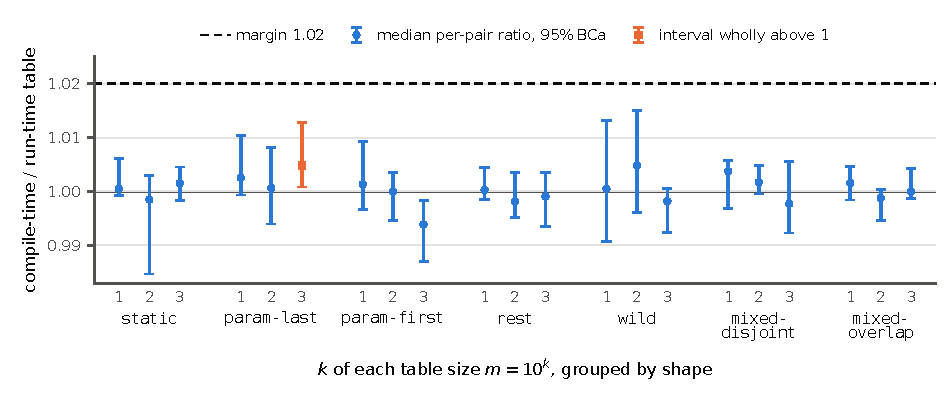
\includegraphics[width=\linewidth]{fig/fig_h7.pdf}
\caption{H7 per cell: the compile-time table's time over the run-time table's, as the median of the
per-pair ratios, with its \Level\% BCa interval. A square marks a cell whose whole interval lies above
one. The dashed line is the margin \Margin.\label{fig:hseven}}
\end{figure}

\begin{table}[htbp]
\caption{H7 per cell. CT and RT are the medians over processes of the compile-time and run-time
tables' times per lookup. ``Upper'' is the upper bound of the \Level\% BCa interval. $X$ counts the
pairs below \Margin, and $p$ is the exact sign test's.\label{tab:hseven}}
\centering\footnotesize\setlength{\tabcolsep}{3.5pt}
\begin{tabular}{@{}llrrrrrrlll@{}}
\toprule
\textbf{Shape} & $m$ & \textbf{CT (ns)} & \textbf{RT (ns)} & \textbf{Ratio} & \textbf{Upper} & $X$ & $p$ &
\textbf{Boot.} & \textbf{Sign} & \textbf{Holds} \\
\midrule
\HSevenRowStaticTen \\ \HSevenRowStaticHundred \\ \HSevenRowStaticThousand \\ \addlinespace
\HSevenRowParamLastTen \\ \HSevenRowParamLastHundred \\ \HSevenRowParamLastThousand \\ \addlinespace
\HSevenRowParamFirstTen \\ \HSevenRowParamFirstHundred \\ \HSevenRowParamFirstThousand \\ \addlinespace
\HSevenRowRestTen \\ \HSevenRowRestHundred \\ \HSevenRowRestThousand \\ \addlinespace
\HSevenRowWildTen \\ \HSevenRowWildHundred \\ \HSevenRowWildThousand \\ \addlinespace
\HSevenRowMixedDisjointTen \\ \HSevenRowMixedDisjointHundred \\ \HSevenRowMixedDisjointThousand \\
\addlinespace
\HSevenRowMixedOverlapTen \\ \HSevenRowMixedOverlapHundred \\ \HSevenRowMixedOverlapThousand \\
\bottomrule
\end{tabular}
\end{table}

\runin{The costs of a compile-time table.} Table~\ref{tab:costs} reports what the tables cost the
compilers. On L, clang \ClangVersion{} compiled each of the \CostTables{} tables in a fresh build, one
job at a time, at the native flags. These are the \CostTablesPerSize{} tables of each size, from the
sixteen table seeds of the run and one more, and the GitHub table. A table's object size is the sum of
its sections named \texttt{.text*}, \texttt{.rodata*}, \texttt{.data.rel.ro*}, the other
\texttt{.data*}, and \texttt{.bss*}. Each object file is \CostPadMin{} to \CostPadMax{} bytes larger.
The page alignment of the table pads the file, without adding memory that the lookup touches.

Clang's need of constant-evaluation steps was measured for the tables of table seed \TableSeedFirst{}
and for the GitHub table. The search doubles the budget from \StepsStart{} steps, so each value is the
smallest budget tried under which a table compiled. Every table of \SizeThousand{} routes compiled
within \ClangNeedMax{} steps and failed at \ClangThousandFailSteps. The budget of \ConstexprSteps{} is
twice the largest of these. On W, an \HostWCpu{} (\HostWArch), MSVC \MsvcVersion{} compiled the same
\MsvcTables{} tables one at a time, with the flags of RegexMatcher's own test of compile-time tables.
Its search starts at \StepsStart{} steps and multiplies by four. At \SizeThousand{} routes every table
crashed the compiler at \MsvcCrashSteps{} steps and failed with the budget error at
\MsvcBudgetFailSteps. Each then compiled at the budget found by halving the last factor of four,
shown in Table~\ref{tab:costs}. At the harness's budget, the compiles of those tables took
\MsvcPeakMinMiB{} to \MsvcPeakMaxMiB~MiB of memory. These are compiler measurements of code that never
runs, so they need no sanitizer record.

\begin{table}[htbp]
\caption{The costs of the compile-time tables: clang on L at the native flags, and MSVC on W, one
compile at a time. Clang's compile time and object size cover every table of a size. The steps and
MSVC's columns cover the tables of table seed \TableSeedFirst{} at each size, and the GitHub table.
Steps are the smallest budget of constant evaluation tried under which a table compiled. Peak memory
is the compiler's peak committed memory at the harness's budget.\label{tab:costs}}
\begin{adjustwidth}{-\extralength}{0cm}
\centering\footnotesize\setlength{\tabcolsep}{4pt}
\begin{tabular}{@{}lrrrrrrr@{}}
\toprule
& & \multicolumn{3}{c}{\textbf{Clang on L}} & \multicolumn{3}{c}{\textbf{MSVC on W}} \\
\cmidrule(lr){3-5}\cmidrule(lr){6-8}
$m$ & \textbf{Tables} & \textbf{Compile (s)} & \textbf{Object (B)} & \textbf{Steps} & \textbf{Steps} &
\textbf{Peak (MiB)} & \textbf{Object file (B)} \\
\midrule
\CostRowTen \\ \CostRowHundred \\ \CostRowThousand \\ \CostRowGithub \\
\bottomrule
\end{tabular}
\end{adjustwidth}
\end{table}

\subsection{Exploratory Runs}\label{sec:exploratory}

The exploratory runs decide nothing and have no intervals (Table~\ref{tab:explore}). On the GitHub
table, v2 took \ExGithubRatio{} of the time of the fastest competitor, \ExGithubFastest, over
\ExGithubPairs{} pairs. It ran \ExGithubVtwoNet{} net instructions per lookup against
\ExGithubFastestNet. With half the queries missing, v2's ratio to the fastest competitor ranged from
\ExMissRatioMin, at \ExMissRatioMinCell, to \ExMissRatioMax, at \ExMissRatioMaxCell. No cell was above
one. v2 ran more net instructions than the fastest competitor in \ExMissNetAbove{} of those cells, all
at $m=\SizeTen$.

Long literals did not close the gap. Their ratios ran from \ExVocabRatioMin{} to \ExVocabRatioMax, and
v2 ran fewer net instructions in all \ExVocabCells{} cells. The Zipf ring gave \ExZipfRatioMin{} to
\ExZipfRatioMax, again with fewer net instructions in every cell. Without decoys, gin holds the
\shape{mixed-overlap} tables, and v2's ratio ran from \ExNoDecoyRatioMin{} to \ExNoDecoyRatioMax{} up
to $m=\SizeTenThousand$. At $m=\ExNoDecoyFailedSize$ the analysis failed that cell. There gin and
Boost.URL agreed in \ExNoDecoyFailOk{} of \RoundTwoReps{} processes and differed as declared in the
others. An arm must agree in all of a cell's processes or in none.

\begin{table}[htbp]
\caption{The exploratory runs, against the fastest competitor of each cell. $R$ is the number of pairs
per cell. ``v2 / fastest'' gives the range over cells of the median over pairs of the per-pair ratio.
The last column counts the cells where v2 ran more net instructions than the fastest
competitor.\label{tab:explore}}
\centering\footnotesize
\begin{tabular}{@{}lrrll@{}}
\toprule
\textbf{Run} & \textbf{Cells} & $R$ & \textbf{v2 / fastest} & \textbf{More instructions} \\
\midrule
GitHub table & one & \ExGithubPairs & \ExGithubRatio & none \\
\ExMissRow \\ \ExVocabRow \\ \ExZipfRow \\ \ExNoDecoyRow \\
\bottomrule
\end{tabular}
\end{table}

The ablation arm shows what the rework of Section~\ref{sec:rework} changed. Against it, v2's lookup time
ranged from \AbTimeMin{} to \AbTimeMax{} of the ablation arm's over the \AbCells{} cells, and its net
instructions were equal (\AbInsnMin). The build took \AbBuildMin{} to \AbBuildMax{} of the ablation
arm's time, and the table's heap bytes were \AbHeapMin{} to \AbHeapMax{} of its bytes.
Appendix~\ref{app:ablation} gives every cell. The rework improved the build time and the heap, and left
the lookup unchanged.
